%# -*- coding: utf-8-unix -*-
%%==================================================
%% thesis.tex
%%==================================================

% 双面打印
\documentclass[master, openright, twoside]{sjtuthesis}
% \documentclass[bachelor, openany, oneside, submit]{sjtuthesis}
% \documentclass[master, review]{sjtuthesis}
% \documentclass[%
%   bachelor|master|doctor,	% 必选项
%   fontset=fandol|windows|mac|ubuntu|adobe|founder, % 字体选项
%   oneside|twoside,		% 单面打印,双面打印(奇偶页交换页边距,默认)
%   openany|openright, 		% 可以在奇数或者偶数页开新章|只在奇数页开新章(默认)
%   english,			% 启用英文模版
%   review,	 		% 盲审论文,隐去作者姓名、学号、导师姓名、致谢、发表论文和参与的项目
%   submit			% 定稿提交的论文,插入签名扫描版的原创性声明、授权声明 
% ]

% 逐个导入参考文献数据库
\addbibresource{bib/thesis.bib}
% \addbibresource{bib/chap2.bib}

\begin{document}

%% 无编号内容:中英文论文封面、授权页
%# -*- coding: utf-8-unix -*-
\title{线程放置策略对层级锁性能和长期公平性影响研究}
\author{赵鹏飞}
\advisor{李健副教授}
% \coadvisor{某某教授}
\defenddate{2019年1月4日}
\school{上海交通大学}
\institute{某某系}
\studentnumber{116037910055}
\major{软件工程}

\englishtitle{Research of Influence of Threads Placement Strategy on Performance and Long-term Fairness of Hierarchical Locks}
\englishauthor{\textsc{Pengfei Zhao}}
\englishadvisor{Prof. \textsc{Jian Li}}
% \englishcoadvisor{Prof. \textsc{Uom Uom}}
\englishschool{Shanghai Jiao Tong University}
\englishinstitute{\textsc{School of Electronic Information and Electrical Engineering} \\
  \textsc{Shanghai Jiao Tong University} \\
  \textsc{Shanghai, P.R.China}}
\englishmajor{Software Engineering}
\englishdate{Dec. 17th, 2018}


\maketitle

\makeatletter
\ifsjtu@submit\relax
	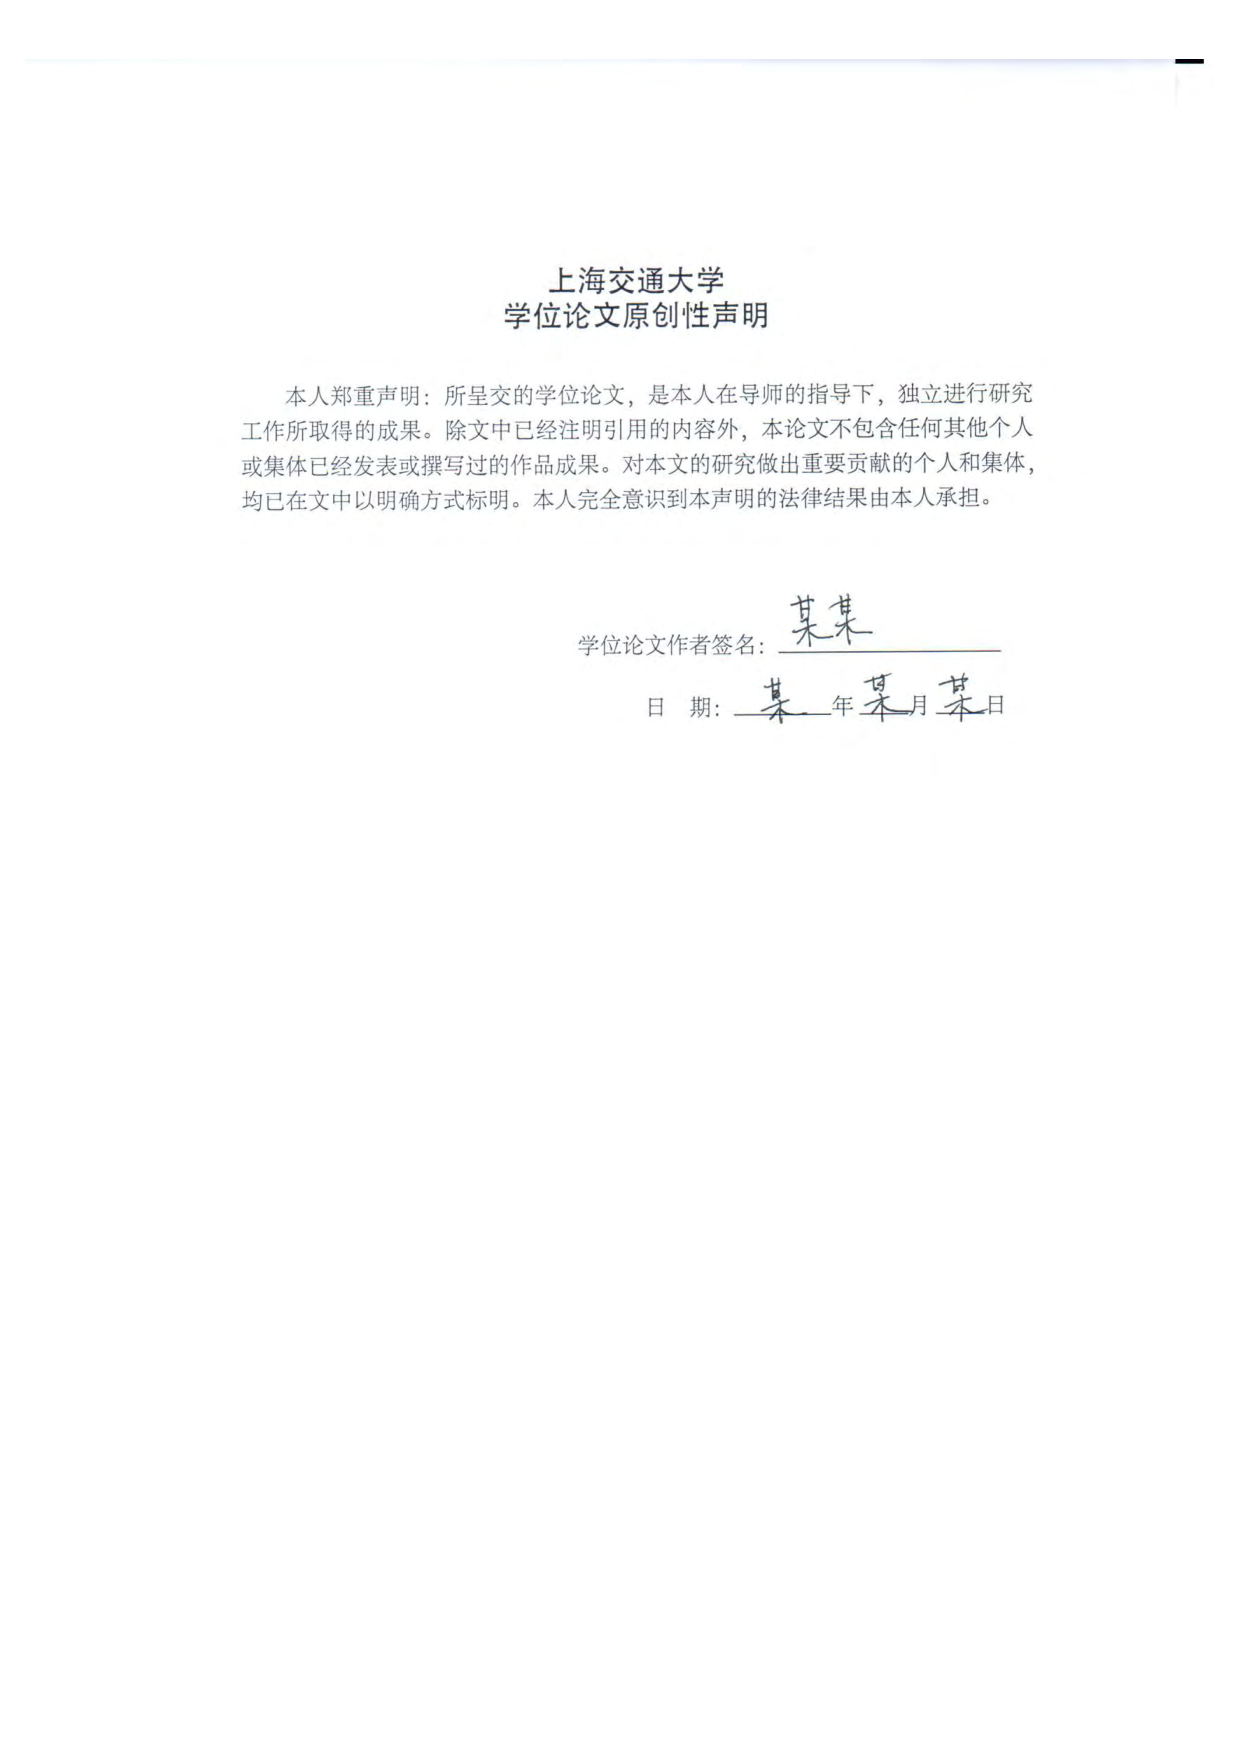
\includepdf{pdf/original.pdf}
	\cleardoublepage
	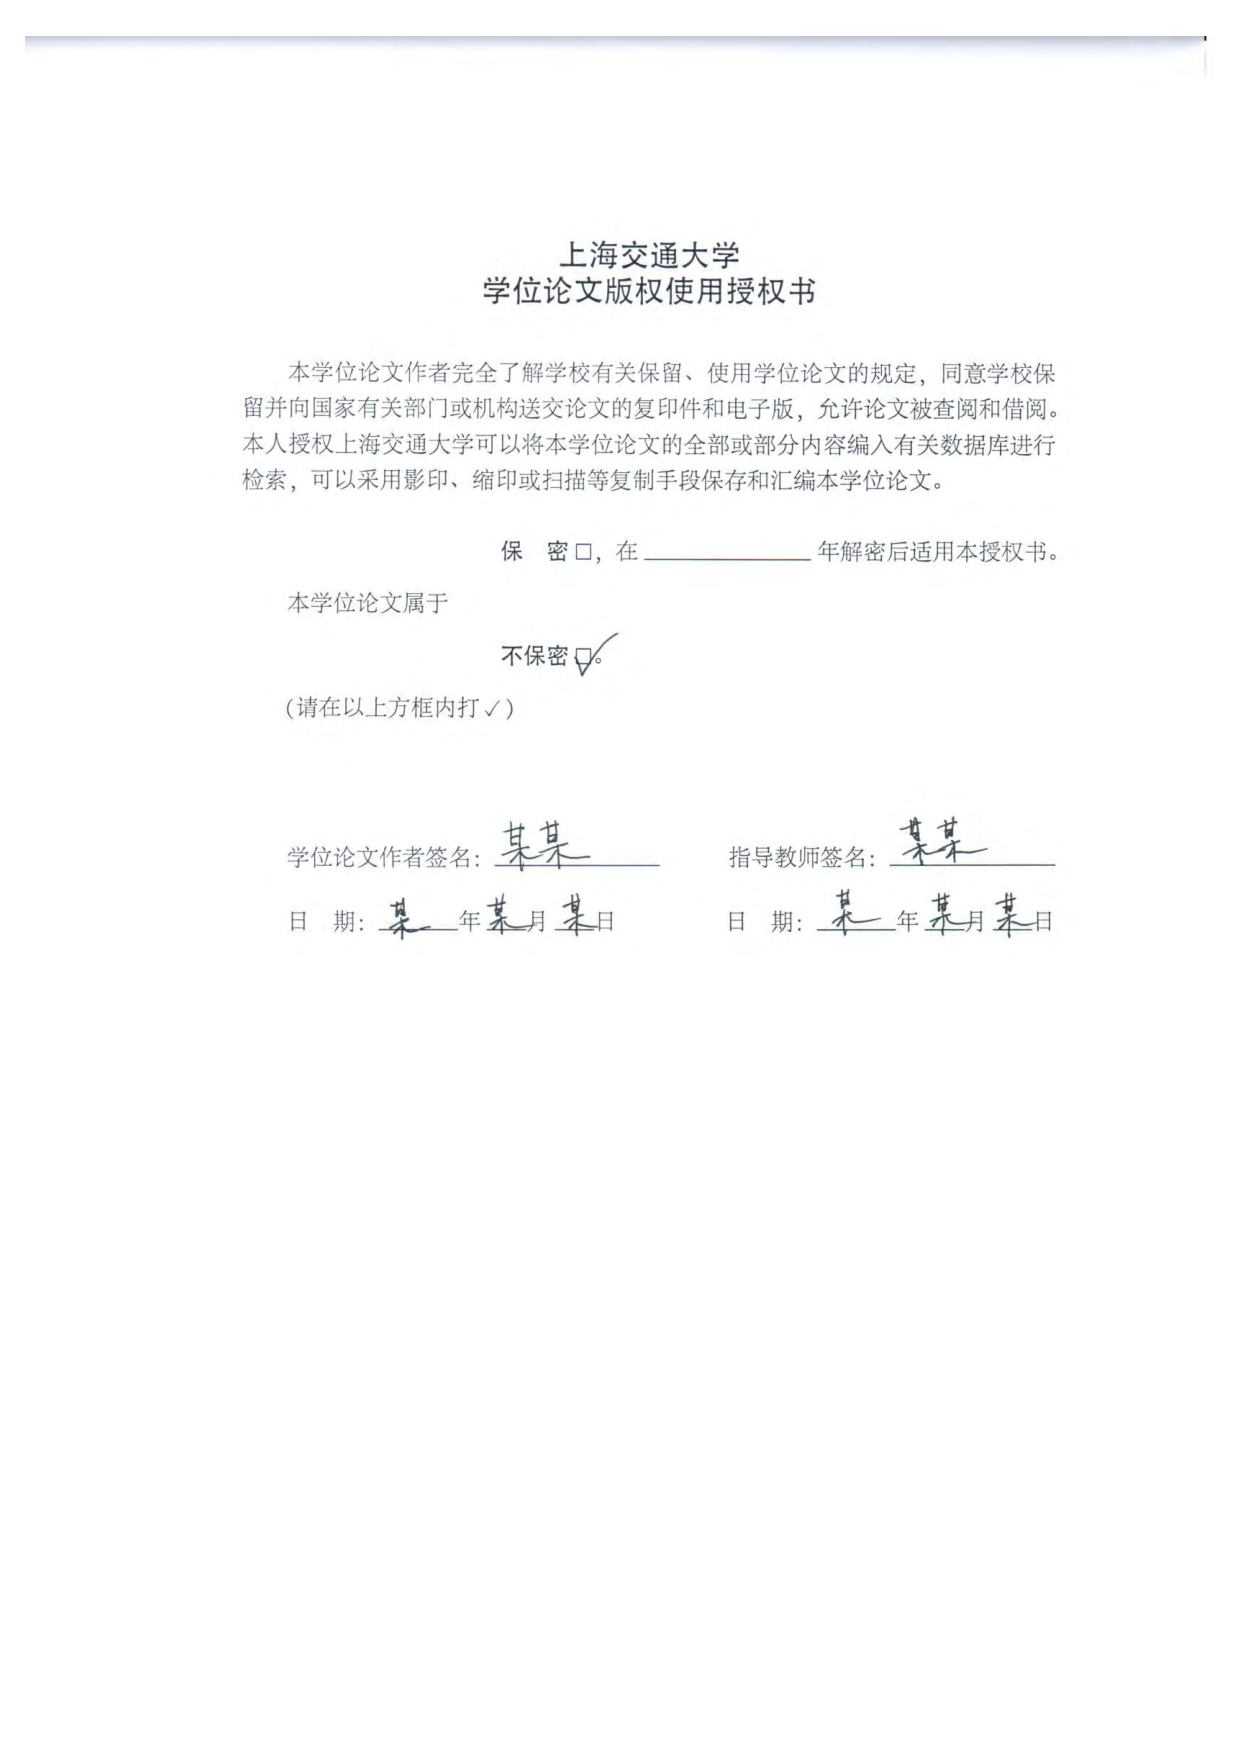
\includepdf{pdf/authorization.pdf}
	\cleardoublepage
\else
\ifsjtu@review\relax
% exclude the original claim and authorization
\else
	\makeDeclareOriginal
	\makeDeclareAuthorization
\fi
\fi
\makeatother


\frontmatter 	% 使用罗马数字对前言编号

%% 摘要
\pagestyle{main}
%# -*- coding: utf-8-unix -*-
%%==================================================
%% abstract.tex for SJTU Master Thesis
%%==================================================

\begin{abstract}
NUMA(Non-Uniform Memory Access, 非一致性内存访问)架构的出现和普及克服了SMP(Symmetric Multi-Processor,对称多处理器)架构在扩展性方面的局限性,使得单台机器上能够容纳更多的计算核心,同时NUMA架构中物理内存的分布式设计也使得访存操作具有非一致性时延的特征。一方面,更多的计算核心使得共享内存的高并发应用能够生成更多的线程并将其分布到所有的核上来充分利用多核资源提高系统吞吐率;另一方面,内存及缓存的非一致性访问特性也使得挖掘和利用共享数据的局部性成为多线程应用获取更高性能的关键。对于极易成为系统性能和扩展性瓶颈的锁来说,线程数的增多和访存的非一致性特征都对其的设计和改进提出了新的挑战。

基于队列的锁,尤其是MCS锁\footnote{命名来源于其作者名字首字母:John Mellor-
Crummey和Michael Scott}和CLH锁\footnote{命名来源于其作者名字首字母:Craig、Landin 和 Hagersten},由于其在性能、可扩展性和公平性方面的良好表现,广泛应用于很多锁集中的高性能系统。这些基于队列的锁通过将参与锁竞争的线程按照其请求锁的顺序排成一个先入先出(FIFO,First In First Out)的队列,每个线程在在队列中各自的内存位置自旋等待锁并且按照其在队列中的顺序依次进入关键区域。FIFO的队列保证了基于队列的锁的公平性,而每个线程在不同的内存位置自旋使其能提供良好的性能和可扩展性。在NUMA架构的机器上,为了充分利用多核资源,竞争同一个锁的线程不可避免地要分布在不同的NUMA节点(node)上,从而产生了跨NUMA节点的锁传递,而访存非一致性特征使得跨节点的锁传递时延通常远大于同一节点内的锁传递时延。传统的基于队列的锁由于不能感知到底层NUMA的特征并且要保持FIFO的锁传递顺序,所以产生了大量的跨节点锁传递,进而产生性能严重下降的问题。

为了解决基于队列的锁在NUMA架构下出现的性能下降问题,NUMA感知的基于队列的层级锁(以下简称层级锁),例如Cohort锁、HMCS(Hierarchical MCS)锁,改变了基于队列的层级锁全局FIFO的锁传递顺序,通过NUMA感知的锁调度使得锁尽可能地在同一个NUMA节点内的线程间按FIFO的顺序传递,只有当当前节点内没有请求者或者锁在当前节点内的传递次数超过一定限度时才将其传给其他节点内的线程,从而减少锁的跨节点传递比例,改善其在NUMA架构下的性能。由于层级锁高性能的获取要依赖于线程在NUMA节点上的分布,因此线程的放置策略对于其最终能达到的性能改善程度有很大影响。现有层级锁中线程通常会被紧凑(Compact)地放置在尽可能少的节点上来减少锁的跨节点传递,这种线程放置策略有利于层级锁挖掘和利用局部性获取更高的性能,但是层级锁优先本地传递的传递机制使得其不能保证长期公平性。除此以外,将线程平均(Even)放置在所有节点上理论上能够保证层级锁的长期公平性,但是由于线程分布较为分散所以在锁的竞争不是很激烈的时候相比紧凑放置又会存在严重的性能下降问题。

现有的简单单一的线程放置策略难以在竞争状况复杂多变的应用中同时保证层级锁的高性能和长期公平性,而对于公有云等应用场景来说,性能和公平性是缺一不可的。在这篇文章中我们提出了一种竞争感知的混合线程放置框架(Contention-Aware Hybrid Threads Placement Framework,以下简称CAH)。在CAH中我们提出了两种新的线程放置策略:有轮换的紧凑放置(Compact With Shift,以下简称CWS)和加强的平均放置(Enhanced Even,以下简称EE)。CWS在紧凑放置的基础上引入了一种轻量级的线程轮换(shift)机制来以极小的性能损失为代价抹平线程之间的吞吐率差异从而使得其能够保证层级锁的长期公平性;EE在平均放置的基础上限制其所能使用的节点数为能放下所有线程的最小节点数而不是所有节点从而在保证长期公平性的前提下尽可能地提高性能。CAH本质上是基于CWS和EE的,能根据应用中层级锁的竞争状况动态调整线程放置策略的一种混合解决方案。它通过定期地取样每个线程的锁相关的事件来评估当前层级锁的竞争状况,并且结合当前的线程数量及其分布来调节线程的放置策略,在层级锁的竞争强度足够高的时候应用EE策略,否则应用CWS策略,从而不论锁的竞争强度如何变化都能以最小的额外代价来同时保证吞吐率和长期公平性。

\keywords{\large 层级锁 \quad 竞争感知的 \quad 长期公平性}
\end{abstract}

\begin{englishabstract}
The emergence of NUMA(Non-Uniform Memory Access) architecture overcomes the scalability limits of SMP(Symmetric Multi-Processor) architecture, enabling more cores integrated on a single machine. While the distributed design of physical memory in NUMA architecture makes memory access suffer from non-uniform latency. More cores enable multithreading applications to use more threads to take advantages of multicore resources and non-uniform memory access latency makes exploiting locality more important to achieve higher performance. Both of these changes in multithreading applications pose new challenges to the design of locks, which tend to become the bottleneck of system performance.

Queue-based locks, especially MCS lock\footnote{after the initials: John Mellor-
Crummey and Michael Scott} and CLH lock\footnote{after the initials:Craig、Landin and Hagersten}, are widely used in lock-intensive high-performance systems due to their good performance on throughput, scalability and fairness. These locks push threads contending for the same lock into a first-in first-out (FIFO) queue by their requesting order. Each thread spins on its own record in the queue and enters critical section by the order in the queue. The FIFO queue guarantees the fairness of queue-based locks, and each thread spinning on a different memory location provides good performance and scalability. On NUMA architecture, in order to make full use of multi-core resources, threads competing for the same lock are inevitably distributed on different NUMA nodes, resulting in inter-node lock transfer, which typically takes much longer time than lock transfer in the same node. The traditional queue-based locks are unaware of  the underlying NUMA factor and they need to maintain the FIFO lock acquisition order. Which involves enormous inter-node lock transfers and thus causes performance degradation.


To avoid performance degradation of queue-based locks on NUMA architecture, NUMA-aware queue-based hierarchical locks (hereinafter referred to as hierarchical locks), such as Cohort locks and HMCS (Hierarchical MCS) locks, change the global FIFO lock transfer order and prefer to transfer the lock to a local waiter in the same node, only if these is no local waiter or the lock acquisitions on local node has exceeded the predefined threshold is the lock transferred to another node. Hierarchical locks reduce the frequency of inter-node lock transfer and thus achieves higher performance under NUMA architecture. Since the high-performance of hierarchical locks depends on the distribution of threads on NUMA nodes, the threads placement strategy has a great impact on the performance improvement that could ultimately be achieved. In existing hierarchical locks, threads are usually placed compactly(Compact Placement) on as few nodes as possible to reduce the frequency of inter-node lock transfer. This strategy helps hierarchical locks exploit locality to achieve higher performance, but the local-preferred lock transfer mechanism of hierarchical locks makes it hard to guarantee long-term fairness. Besides, placing threads evenly on all nodes(Even Placement) theoretically guarantees the long-term fairness of hierarchical locks, but since the thread distribution is more sparse, when the lock contention is not high enough, it could lead to serious performance degradation compared to Compact placement.

The existing threads placement strategies in hierarchical locks could not guarantee both high throughput and long-term fairness or could only guarantee both of them when highly contended. While in some scenarios such as public cloud both throughput and fairness is key to success and the lock contention could vary from time to time. In this paper, we present a contention-aware hybrid threads placement framework CAH.   In CAH we propose two new thread placement strategies: Compact With Shift (CWS) and Enhanced Even (EE). CWS introduces a lightweight thread shifting mechanism into compact placement to smooth the throughput difference among threads. EE limits the number of nodes even placement could exploit to the minimum number of nodes that could place all threads, instead of all nodes. CAH is essentially a hybrid solution of CWS and EE that dynamically adjusts the thread placement strategy based on the lock contention in the application. When the contention level of the lock is high enough, CAH applies EE strategy, otherwise CWS strategy, so that regardless of the change of lock contention, the throughput and long-term fairness could always be guaranteed.

\englishkeywords{\large hierarchical locks, threads placement, contention-aware}
\end{englishabstract}



%% 目录、插图目录、表格目录
\tableofcontents
\listoffigures
\addcontentsline{toc}{chapter}{\listfigurename} %将插图目录加入全文目录
\listoftables
\addcontentsline{toc}{chapter}{\listtablename}  %将表格目录加入全文目录
\listofalgorithms
\addcontentsline{toc}{chapter}{\listalgorithmname} %将算法目录加入全文目录

%# -*- coding: utf-8-unix -*-
\begin{nomenclaturename}
\label{chap:symb}

\begin{longtable}{rl}
$\epsilon$     & 介电常数 \\
 $\mu$ 		& 磁导率 \\
 $\epsilon$     & 介电常数 \\
 $\mu$ 		& 磁导率 \\
 $\epsilon$     & 介电常数 \\
 $\mu$ 		& 磁导率 \\
 $\epsilon$ 	& 介电常数 \\
 $\mu$ 		& 磁导率 \\
 $\epsilon$     & 介电常数 \\
 $\mu$ 		& 磁导率 \\
 $\epsilon$     & 介电常数 \\
 $\mu$ 		& 磁导率 \\
 $\epsilon$     & 介电常数 \\
 $\mu$ 		& 磁导率 \\
 $\epsilon$ 	& 介电常数 \\
 $\mu$ 		& 磁导率 \\
 $\epsilon$     & 介电常数 \\
 $\mu$ 		& 磁导率 \\
 $\epsilon$     & 介电常数 \\
 $\mu$ 		& 磁导率 \\
 $\epsilon$     & 介电常数 \\
 $\mu$ 		& 磁导率 \\
 $\epsilon$ 	& 介电常数 \\
 $\mu$ 		& 磁导率 \\
 $\epsilon$     & 介电常数 \\
 $\mu$ 		& 磁导率 \\
 $\epsilon$     & 介电常数 \\
 $\mu$ 		& 磁导率 \\
 $\epsilon$     & 介电常数 \\
 $\mu$ 		& 磁导率 \\
 $\epsilon$ 	& 介电常数 \\
 $\mu$ 		& 磁导率 \\
 $\epsilon$     & 介电常数 \\
 $\mu$ 		& 磁导率 \\
 $\epsilon$     & 介电常数 \\
 $\mu$ 		& 磁导率 \\
 $\epsilon$     & 介电常数 \\
 $\mu$ 		& 磁导率 \\
 $\epsilon$ 	& 介电常数 \\
 $\mu$ 		& 磁导率 \\
 $\epsilon$     & 介电常数 \\
 $\mu$ 		& 磁导率 \\
 $\epsilon$     & 介电常数 \\
 $\mu$ 		& 磁导率 \\
 $\epsilon$     & 介电常数 \\
 $\mu$ 		& 磁导率 \\
 $\epsilon$ 	& 介电常数 \\
 $\mu$ 		& 磁导率 \\
 $\epsilon$     & 介电常数 \\
 $\mu$ 		& 磁导率 \\
 $\epsilon$     & 介电常数 \\
 $\mu$ 		& 磁导率 \\
 $\epsilon$     & 介电常数 \\
 $\mu$ 		& 磁导率 \\
\end{longtable}

\end{nomenclaturename}
 % 主要符号、缩略词对照表

\mainmatter	% 使用阿拉伯数字对正文编号

%% 正文内容
\pagestyle{main}
%# -*- coding: utf-8-unix -*-
%%==================================================
%% chapter01.tex for SJTU Master Thesis
%%==================================================

%\bibliographystyle{sjtu2}%[此处用于每章都生产参考文献]
\chapter{绪论}
\label{chap:intro}


\section{研究背景和意义}
近年来,NUMA(Non-Uniform Memory Access,非一致性内存访问)\cite{feliu2012understanding}\cite{dashti2013traffic}架构的服务器逐渐普及,它的出现解决了对称多处理器(symmetric multiprocessor architecture,SMP)架构在可扩展性方面的局限性\cite{pusukuri2014shuffling},所以已经成为现代服务器架构设计中的一种趋势和规范\cite{kashyap2017scalable}\cite{chabbi2016contention}\cite{chabbi2017efficient}。良好的可扩展性使得单个NUMA架构的机器上可以轻易集成更多的计算核心,更大容量的物理内存和更大的内存访问带宽。NUMA架构中计算、存储等资源被组织成若干节点(node),每个节点包括若干计算核心,一块物理内存,一个或多个内存访问控制器(memory controller)和多层缓存,计算节点之间通过高速芯片间通信介质连接。在NUMA架构的机器中,某个计算核心访问其所在的计算节点的本地内存,尤其是本地共享缓存的速度通常是访问在其他计算节点上的内存或缓存的速度的数倍,也就是说NUMA架构的机器中内存访问存在非一致性时延。另外,在同一个计算节点内部,由于缓存的的分层设计,同一个计算核心访问本地计算节点的不同层次的缓存也会有显著的非一致性时延\cite{chabbi2015high}。

对于大型内存数据库(例如Microsoft SQL server)\cite{MICROSOFT-SQL}和处理引擎\cite{SAP}\cite{zaharia2010spark}(例如spark)等通过高并发来处理大规模海量数据的应用来说,随着数据规模的指数增长,必然需要进一步地扩展,通过更高程度的并发来满足需求。而NUMA架构提供的更多的核,更大的内存容量和更大的内存访问带宽使得这些应用可以生成更多的线程,并将这些线程分布到所有的NUMA计算核心上来尽可能地利用所有NUMA节点的计算和存储资源。另一方面,NUMA架构本身存在的内存访问的非一致性时延以及NUMA节点之间的有限的带宽资源对系统的线程调度和内存管理提出了新的挑战\cite{wang2012performance}\cite{boyd2008corey}。这些共享内存的应用中线程之间通常存在大量的共享数据,数据在内存及缓存中的存储位置和及访问该数据的线程的在机器上执行位置决定了数据访问的效率,因而对于系统的整体性能有很大影响。合理的内存管理和线程调度能够充分利用数据访问的局部性提高性能,而不合理的内存管理和线程调度策略可能会造成整体性能的严重损失。

通过挖掘应用的数据访问特征,比如线程线程和线程之间的数据共享范围和共享频率来建立线程之间的亲和性(thread affinity)及线程与数据之间的亲和性(data affinity)\cite{diener2014kmaf}\cite{azimi2009enhancing}\cite{tikir2008hardware},然后将共享数据多共享频率高的线程对调度到相同的NUMA节点上,同时将其最常访问的数据也放置在该NUMA节点上,可以充分利用数据访问的局部性来减少数据拷贝,减少缓存更新、增加缓存的利用率和命中率,降低数据访问延迟,进而提高应用的整体性能\cite{chishti2005optimizing}。除了将数据迁移到经常访问其的NUMA节点(co-location)外,通过分析数据本身的特征,比如读写比、共享范围、访问来源(来自于哪个NUMA节点)等,并且考虑NUMA节点间高速通信介质的数据传输压力及NUMA节点上内存控制器访问压力等因素后,还可以通过其他的内存管理方式来提高系统性能\cite{dashti2013traffic}\cite{molka2011memory},比如对于共享范围很大的只读数据或者读写比非常高的数据可以通过在NUMA节点之间复制(replication)该数据来减少跨节点的数据访问;对于访问来源非常分散的共享热点数据可以通过将数据交织(interleaving)分布到各个NUMA节点来分摊内存控制器的访问压力;对于某些应用可以将数据放置在第一次(first-touch)访问其的线程所在NUMA节点来利用局部性等。

在线程之间所有共享的数据中,有部分特殊数据不能被多个线程同时访问因而需要一种同步机制来防止其被同时访问更新,尽管近年来事务内存(transaction memory)开始流行,但是对于多数高并发的应用来说,在高度竞争的情况下锁依然是一种最基本最重要并且广泛使用的同步机制\cite{tallent2010analyzing}\cite{johnson2010decoupling}。NUMA架构的出现对于锁的性能影响主要有三个方面:1)锁本身及其保护的数据都是线程之间的共享数据,这部分数据在所有共享数据中占比通常很小,并且通常读写比很低,所以内存管理(迁移,复制,交织等)对其性能基本没有影响,而线程调度会影响对其性能仍有重要影响;2)线程之间对于锁及其保护的数据的在时间上是不共享的,而这部分数据的访问顺序是由线程的拿锁顺序决定大的,所以通过线程调度优化锁的性能还必须考虑锁本身的传递机制;3)(互斥)锁保护的数据只能在线程间串行访问,这使得锁很容易成为应用的性能瓶颈甚至导致应用崩溃\cite{boyd2012non},NUMA因素的出现进一步加剧了这种瓶颈,也对锁的设计提出了新的挑战。

在传统的SMP架构中,基于队列的锁,例如CLH锁\cite{craig1993building}\cite{magnusson1994queue}\cite{scott2013shared}和MCS锁\cite{mellor1991algorithms}\cite{scott2013shared},广泛应用在许多锁集中的高性能系统中\cite{dice2011flat}。这些基于队列的锁将所有等待访问关键区域的线程排成先进先出(FIFO,first in first out)的队列,每个线程通过在队列中各自对应的内存位置上自旋来等待进入关键区域。相比所有线程在同一个内存位置上自旋的spin lock, FIFO的队列保证了基于队列的锁的公平性;每个线程在各自的内存位置上自旋,分散了线程对锁变量的竞争,减少了锁传递时的缓存更新,从而提能提供更好的性能和可扩展性。然而在NUMA架构中,这些基于队列的锁的性能显著下降,这主要是由NUMA架构机器的物理架构决定的,由于传统的基于队列的锁不能感知NUMA架构硬件层面的访存的非一致特性,同时为了保持先来先服务的锁传递顺序,就会产生锁在NUMA节点之间的随意传递,而锁在NUMA节点之间的传递地时延通常是在同一个NUMA节点内传递时延的数倍,从而加长锁传递的时间和关键区域的执行时间,增加时延,减小吞吐率,使得性能显著下降。

传统锁在NUMA架构上性能衰退的主要原因是跨节点的锁传递代价远高于同一节点内的锁传递代价而传统锁不能感知到底层的NUMA因素。NUMA感知的层级锁在考虑NUMA因素的情况下通过本地偏好的锁传递规则减少了锁的跨节点传递,从而改善了锁在NUMA架构下的性能表现。本文在此基础上从线程调度/放置策略的角度对现有的基于队列的层级锁的性能和其他特性(长期公平性)进行优化,使其能够更好地适应诸如公有云等对于锁的性能,公平性,可扩展性等都有很高要求的应用场景。

NUMA架构是可预见的未来大型计算机硬件架构设计的大趋势,而随着医疗,交通,社交等领域产生的大数据的爆发式的增长,以及云计算等共享计算资源模式的快速发展,大型应用对于性能,可扩展性和公平性等方面的要求必然进一步提高。本文的研究使得基于队列的层级锁能够更好地适应未来软硬件的特性和需求变化,更好地服务于当下和未来相关领域的发展。总而言之,NUMA架构的出现解决了大型计算机硬件层面的扩展性问题,使得高性能共享内存应用能够进一步地扩展来满足日益增长的数据处理的需要;层级锁的出现改善了基于队列的锁在NUMA架构下存在的性能衰退问题,但是也带来了长期公平性不足的新问题;而本文的研究从线程调度/放置的角度进一步地优化现有的层级锁设计,使其在保持性能和可扩展性的前提下在一定程度上保证公平性。考虑到NUMA架构的机器的不断普及以及发展趋势和公有云等对公平性,性能和可扩展性都有很高要求的应用场景的不断增多,本文的研究将使得层级锁能够更好适应这些应用场景的需求,并且在可预见的未来有更大应用前景。
\section{国内外研究现状}
性能和公平性是任何锁的设计中都必须要考虑的两个重要标准\cite{chabbi2015high}。一般情况下,线程执行关键区域的时间非常短,甚至可能比其拿锁的时间还要短\cite{johnson2010decoupling},所以锁传递的时延对于锁的性能尤其是在锁的竞争已经饱和的情况下的性能的影响非常大。而在NUMA架构下,访存的非一致性时延特征导致跨节点的锁传递和同一节点内的锁传递在时延方面存在数倍的差异,从而使得跨节点的锁传递比例成了影响锁性能的关键因素。针对NUMA架构下跨节点的锁传递带来的锁性能下降问题,现有的优化方案大多数本质上都是通过减少锁的跨节点传递来改善其性能的,具体分为以下四类,即委托执行,线程聚类,线程迁移,NUMA感知的层级锁。另外,应用程序在NUMA架构下的进一步扩展使得其对锁的竞争变得更加难以预测,过度的竞争反而会带来系统整体性能的下降,所以通过竞争控制也能改善NUMA架构下锁的性能。

\subsection{委托执行}
为了避免锁在NUMA节点之间传递的巨大开销,要执行关键区域的线程可以委托一个或几个专门的核代为执行\cite{oyama1999executing}\cite{lozi2012remote}\cite{fatourou2012revisiting}\cite{hendler2010flat}\cite{guiroux2016multicore},从而完全避免锁的传递所造成的缓存数据的同步及由此带来的时延增加和吞吐率损失,因为锁及其保护的数据始终在对应核的缓存中。这种方案的代价是需要额外的线程间通信并且至少需要一个专用的核专门执行关键区域。RCL(remote core locking)\cite{lozi2012remote}就是委托执行的一种,RCL的作者观察到大多数多线程应用并不需要或者不能扩展到现代多核机器的所有核上,所以让某几个特定的核专门执行关键区域既利用了空余的核又能带来潜在的性能提升,要执行关键区域的线程不需要通过竞争锁来进入关键区域,而是通过优化后的远程过程调用委托特定核完成关键区域的执行从而完全避免锁及其保护的数据的传递。委托执行本质上是在迁移关键区域的执行,相比其他锁,它能在某些特定应用中防止高度竞争情况下应用性能的崩溃,但是它最大的缺陷是需要修改使用传统锁的历史遗留代码,原有代码中的关键区域需要额外的技术和时间被识别和修改之后才能利用委托执行的的高性能。

\subsection{线程聚类}
线程聚类是把同一个应用的线程或者竞争同一个锁的线程放置到同一个NUMA节点上\cite{tam2007thread}\cite{thekkath1994impact}\cite{xian2008contention}。这样做的好处是所有的共享数据都存在于本地内存或者缓存中,并且将锁的传递限制在同一个NUMA节点内部,避免了锁在NUMA节点之间传递的开销。该方案本质上是通过建立线程间的亲和性来挖掘和利用数据访问的局部性,所以也常被用在一般的共享数据中将有共享内存数据的线程放置在同一个计算节点上来最大化缓存的共享和复用。线程聚类能显著改善线程较少的小规模应用
的性能,但是对于具有大量线程的高并发应用程序而言,其所拥有的线程数通常远大于单个节点上的计算核心,按照线程聚类的方法所有线程都会被分到一个聚类中,因而会产生负载不均衡的问题,同时并行性也被牺牲了,除此以外也会带来拿锁者被抢占或者等待者被抢占等新问题,最终的结果可能得不偿失,所以线程聚类一般只适用于线程数量较少的小规模应用。

\subsection{线程迁移}
在系统运行的同时,将锁的等待者动态地调度到锁的持有者当前所在NUMA节点上,从而减少锁及关键区域的数据在NUMA节点之间的传递\cite{sridharan2006thread}\cite{thekkath1994impact}。这种方案主要基于以下观察,即锁集中的多线程应用的性能对于线程在NUMA节点之间的分布高度敏感但是操作系统的调度器感知不到锁在线程之间的竞争自然不能将锁的竞争因素加入到调度器的调度策略中,所以线程迁移可以看作是在考虑锁竞争因素的情况下对操作系统默认调度器调度策略的一种补充。shuffling\cite{pusukuri2014shuffling}是通过线程迁移来提高锁的性能的一种,它定期地将线程按照其“到达时间”(线程请求锁的时间)来排序;然后将“到达时间”接近的线程分到同一组中,每组的线程数量大致等于单个NUMA节点上的计算核心数;最后将分到同一组的线程迁移到同一个NUMA节点上去执行。因为连续请求锁的线程被分为同一组并且放到同一个节点上执行,所以锁在节点之间的迁移频率被显著降低;另外放置在每个计算节点上的线程数不超过该节点上的计算核心数又能避免负载不均衡及抢占等问题。线程迁移能够有效减少锁及关键区域的迁移,提高系统的整体性能,并且不改变原有锁的传递顺序,代价则是较为频繁大量的线程迁移及其带来的潜在缓存污染等问题。

\subsection{NUMA感知的层级锁}
层级锁利用多层的锁来对应下层的NUMA结构,将锁的竞争分割在不同的NUMA节点或者同一个NUMA节点内部不同的计算核心上,从而减少锁及关键区域数据在NUMA节点间的随意迁移频率\cite{dice2012lock}。与其他解决方案的主要不同之处在于层级锁是对锁的调度,所以会改变原有锁的传递顺序。层级锁本质上是通过牺牲短期公平性来换取减少锁的跨节点传递频率提高锁的吞吐率的。具体来说,在层级锁中,锁的持有者会优先将锁传递给当前节点上的最早的请求者而不是所有节点范围内的最早的请求者,只有当前节点上没有请求者时才会传给其他节点上的请求者。另外为了避免饥饿(starvation)及深度不公平等问题,层级锁中通常会设定一个上限(threshold)来限制其在同一个节点内的连续传递次数。

现有的层级锁设计方案包括lock cohorting\cite{dice2012lock}, HMCS锁\cite{chabbi2015high},AHMCS锁\cite{chabbi2016contention}和HMCS-T\cite{chabbi2017efficient}等。lock cohorting的设计包括一个全局锁(global lock)和每个NUMA节点上的本地锁(local lock)。全局锁和本地锁都可以是任何传统的锁(MCS, CLH,门票锁,自旋锁等)。全局锁在所有节点之间共享,它的主要功能是将竞争分隔到各个节点之内。一个本地锁只在本地节点里边的线程之间共享并且用来同步本地节点内的线程。一个线程只有同时拿到全局锁和其所在节点的本地锁才可以访问关键区域,通常的拿锁顺序是先拿本地锁再拿全局锁。层级锁一般用在竞争线程多竞争激烈的场景中,所以大多数情况下同一个NUMA节点内的线程只需要有一个线程显式拿全局锁另一个线程显式放全局锁,其他线程直接继承全局锁。由于只有全局锁会在节点之间传递并且该传递频率因为竞争分割的关系会很低,所以锁的整体性能显著提高。

HMCS将lock cohorting的思想推广到了具有深层NUMA架构的机器中,从而使用三层甚至四层地MCS锁来潜在地发掘和利用各个NUMA层次的局部性获取更高的性能。HMCS适合竞争线程多竞争锁请求频繁的场景,但是竞争强度较小或者没有竞争的场景下,其多层的锁架构会带来较大的时延。AHMCS针对该问题使用多个互相正交的策略(事务性内存,竞争感知、动态适应的锁树等)来同时达到高竞争时的高吞吐和低竞争时的低时延。HMCS-T保持了HMCS的高性能,并且通过超时机制来使HMCS具备放弃竞争特性从而控制竞争者数量避免无意义的空转等待。由于基于队列的MCS锁相比自旋锁、门票锁等在高度竞争地场景下具有性能好,可扩展性好,并且保证公平性等优点,所有大多数层级锁中将MCS锁作为其各层的基本锁。上述层级锁具有不同的其他方面地特征和创新,但它们都是通过竞争分割降低锁的跨节点传递频率来提高锁的吞吐率的。

\subsection{竞争控制}
许多并行程序的线程之间的通信变化是不可预测的,这使得线程对于共享数据的竞争无法预测和控制,从而使得大多数情况下表现良好的锁可能因为线程对共享数据的竞争的突然加剧而性能急剧下降甚至崩溃\cite{johnson2010decoupling}\cite{boyd2012non}。在NUMA架构下,如前所述,硬件的扩展使得软件应用规模进一步加大,从而使得共享数据的竞争更加不可预测和控制,也进一步加大了应用性能下降和崩溃的风险,所以通过控制线程对于共享数据的竞争也可以改善NUMA架构下锁的性能。

F.Ryan Johnson\cite{johnson2010decoupling}认为通过自旋(spinning)能够最大化锁的性能但是会白白浪费计算资源,而基于阻塞(blocking)的方式节省了计算资源但是可能会加长关键区域的执行时间,同时在高度竞争或者负载变化的情况下,操作系统的调度造成的线程被抢占进一步加剧了上述两种竞争控制策略的缺陷。作者观察到竞争控制与线程调度或者负载管理带来的问题之间是正交的,所以将两者解耦能够更有效的解决两者带来的问题,基于此提出了一种与竞争大小相解耦的的负载控制机制来控制活跃线程数,从而能结合利用spinning的高效性和blocking大的健壮性。类似的,CST锁\cite{kashyap2017scalable}中作者认为简单的spin,block或者spin-then-block竞争控制机制都不能解决NUMA架构下锁存在的扩展性问题,因为不管哪种机制都会受到操作系统调度器的调度决策的影响,所以提出在锁传递的时候在尽可能地保证先来先服务(first-in first-out)的顺序下应该尽可能地将锁传给处于spinning状态的竞争者,从而尽可能地避免因为线程调度而加长关键区域的执行时间。

AHMCS\cite{chabbi2016contention}锁中,作者认为NUMA架构下可扩展性和性能都很好地HMCS\cite{chabbi2015high}锁不能适应竞争和负载多变的环境。HMCS锁在高竞争的情况下能够利用局部性感知提供高吞吐率,但是在竞争很小地情况下局部性感知本身没有必要而且为了进行局部性感知会造成不必要的额外时延,在此基础上作者认为局部性感知的锁应该是竞争感知的,并且提出了可以动态适应竞争变化,动态改变锁的层数的AHMCS锁,从而使其能够在高度竞争的情况下保持高吞吐率的同时在竞争强度不高时也能保证低时延。

Multhusian锁\cite{dice2017malthusian}的作者认为现代大型应用程序大多数使用了过多的线程(overthreaded),大部分这类程序中由于锁的高度竞争,过多的线程非但没有提高应用的性能,反而可能因为扩展性崩溃(scalability collapse)而造成性能衰退。作者通过实验说明了大多数应用中,随着线程数的增多,在锁饱和前性能就开始衰退了,所以使锁饱和的线程数可以用来作为竞争控制的目标。为了将线程数控制在饱和点附近,作者对MCS锁的传递机制进行了修改,借用了内存管理中的thrashing机制\cite{denning1980working}将所有线程分为了活跃态(可以请求锁)和抑制态(不能请求锁)两个集合,其中处于活跃态的线程数大约等于锁的饱和点大小,从而有效控制了竞争线程数进而保证性能不会下降太多。该方案事实上通过牺牲MCS锁的短期公平性来放置性能下降,为了保证长期公平性,作者使用了shift机制来在两个集合之中循环移动线程。

\section{研究内容和结构安排}
本文的研究在基于队列的层级锁基础上,针对现有层级锁中的简单单一的线程放置策略不能在锁的竞争复杂多变的情况下同时保证其性能和长期公平性的缺陷,提出了一种新的竞争感知的混合线程放置框架,使得基于队列的层级锁能够在竞争状况变化的情况下以尽可能小的代价同时达到高性能和保证长期公平性。


\subsection{竞争感知的混合调度框架}
性能和公平性是任何锁设计中最重要的两个指标,而目前的层级锁设计及其线程放置策略或者不能保证最佳的性能,或者不能保证线程之间的长期公平性,或者只能在高竞争的情况下同时保证性能和公平性。究其原因主要有两点:1)现有部分线程放置策略没有考虑对性能和长期公平性都有很高要求的应用场景;2)简单单一的线程放置策略难以满足复杂多变的应用竞争状况。对于公有云等很多应用场景来说,为了给用户提供按需付费的服务并且高效地利用计算、存储等资源,性能和公平性对于其的成功都是至关重要的\cite{rao2014towards};另外,很多大型应用中线程之间对于共享资源的竞争是不可预测和控制的,通常情况下竞争很小的一块共享数据可能会突然变得高度竞争,比如搜索引擎中突然出现的热门事件的搜索\cite{chabbi2016contention}。所以为了适应这些复杂应用场景的需求,现有的基于队列的层级锁的线程放置策略必须要先解决上述两个缺陷/挑战。

基于此,本文的研究首先针对紧凑放置不能保证长期公平性和平均放置性能较差的问题对其分别做了改进,对应得到以下两种新策略,加强的平均放置(Enhanced Even,EE)和有轮换的紧凑放置(Compact With Shift,CWS)
\begin{itemize}
\item 加强的平均放置。为了尽可能地保证平均放置的性能,我们限制该策略所能使用的NUMA节点数为能满足需要的最少的节点数,而不是全部可用的节点数。相比原有的平均放置策略,新的策略在保证长期公平性的同时尽可能地保存局部性使得层级锁能尽可能地挖掘局部性从而保证高性能,然而相比紧凑放置,新的策略在某些情况(竞争强度不足)下还是会有相当的性能损失。
\item 有轮换的紧凑放置。我们发现紧凑放置之后每个线程的吞吐率是由其所运行的位置决定的,所以在紧凑放置的基础上,引入了轮换(shift)机制,即通过定期地交换线程的位置来抹平线程的吞吐率之间的差异从而保证长期公平性。在有轮换的紧凑放置策略中,轮换的频率决定了最终的长期公平性的好坏。
\end{itemize}
基于上述两种改进后的策略及应用程序竞争状况复杂多变的特征,我们提出了竞争感知地混合线程放置框架(Contention-Aware Hybrid Thread Placement Framework)CAH。相比现有的简单单一的线程放置策略,CAH主要有以下几个特征:
\begin{itemize}
\item 竞争感知,该框架通过取样检测锁事件来评估当前的竞争状况,从而能够适应复杂多变的程序竞争状况。其中锁事件是每个线程与锁相关的操作(请求锁,拿锁,放锁)。
\item 混合,该框架可以被看作是有轮换的紧凑放置和加强的平均放置的混合体,在竞争强度足够的情况下应用加强的平均放置否则应用有轮换的紧凑放置策略,最终的目的是用最小的代价同时保证层级锁的性能和长期公平性。
\item 动态,该框架按照应用中层级锁的复杂多变的竞争状况动态地应用合适的线程放置策略。
\end{itemize}

在特定应用中特定的竞争状况下,为了确定一个最合适线程放置策略,我们从Malthusian锁中引入了饱和点(saturation point)的概念。饱和点是能保证某个线程放锁时总有至少一个其余线程在等锁的最小线程数。我们的线程放置框架偏向于应用加强的平均放置策略,因为相比有轮换的紧凑放置策略它没有额外的线程迁移开销。针对某个特定的竞争状况,如果采用加强的平均放置策略后,每个NUMA节点上的线程数大于饱和点,则能在保证长期公平性的情况下获取高性能,所以应用加强的平均放置策略,否则应用有轮换的紧凑放置策略。
\subsection{结构安排}
本文共分为五个章节,具体如下:

第一章为绪论,主要概括介绍了本文的研究背景、意义及本文的研究内容。本文大的研究大背景主要是NUMA架构的扩展性和访存的非一致性带来的新的机遇和挑战,尤其是NUMA架构给现有锁设计带来的挑战。本文的研究基于NUMA感知的基于队列的层级锁,对基于队列的层级锁中现有线程放置策略进行了改进并提出了一种竞争感知的混合线程放置框架使其能够在应用中锁竞争复杂多变的场景下同时保证性能和长期公平性。

第二章介绍了相关研究和技术。包括NUMA架构的特征及相关优化技术,MCS锁、C-MCS锁的算法及其相比其他锁的优缺点,基于队列的层级锁中现有的线程调度/放置策略及其适应场景等。

第三章在对层级锁的锁传递机制及现有线程放置策略做了详细分析,并配合相关的实验验证后,发现现有的线程放置策略的设计初衷对于保证锁的性能或长期公平性是充分而不必要的,在此基础上分别针对现有的两种线程放置策略提出了相应的改进思路,并在这两种改进思路的基础上提出了一套在保证锁的性能和长期公平性的前提下额外开销尽可能小的综合线程放置方案,即竞争感知的混合线程放置框架CAH。

第四章详细阐述了本文研究的竞争感知的混合线程放置框架CAH的架构设计和实现。其中CAH的设计方面包括基本的设计思路即CAH如何解决现有线程放置方案存在的缺陷、CAH的架构和核心算法。CAH的实现主要包含了线程迁移,策略切换等的实现细节。

第五章通过在microbenchmark stress\_one和实际应用memcached上的实验说明了本文的两个改进线程放置策略及CAH整体相对层级锁中原有线程放置策略的有效性。

第六章对全文进行了总结和展望。
\section{本章小结}
本章首先介绍了NUMA架构的基本特征及其对于多线程高性能软件设计尤其是锁带来的机遇和挑战,然后介绍现有研究针对传统锁在NUMA架构下性能下降所做的改进(主要是基于队列的层级锁),接着分析了现有层级锁中线程放置策略存在的优缺点,最后基于现有线程放置策略相应提出了本文的研究内容:针对基于队列的层级锁的竞争感知的混合线程放置框架。
%# -*- coding: utf-8-unix -*-
%%==================================================
%% chapter02.tex for SJTU Master Thesis
%% based on CASthesis
%% modified by wei.jianwen@gmail.com
%% Encoding: UTF-8
%%==================================================

\chapter{{\LaTeX} 排版例子}
\label{chap:example}

\section{列表环境}
\label{sec:list}

\subsection{无序列表}
\label{sec:unorderlist}

以下是一个无序列表的例子,列表的每个条目单独分段。

\begin{itemize}
  \item 这是一个无序列表。
  \item 这是一个无序列表。
  \item 这是一个无序列表。
\end{itemize}

使用\verb+itemize*+环境可以创建行内无序列表。
\begin{itemize*}
  \item 这是一个无序列表。
  \item 这是一个无序列表。
  \item 这是一个无序列表。
\end{itemize*}
行内无序列表条目不单独分段,所有内容直接插入在原文的段落中。

\subsection{有序列表}
\label{sec:orderlist}

使用环境\verb+enumerate+和\verb+enumerate*+创建有序列表,
使用方法无序列表类似。

\begin{enumerate}
  \item 这是一个有序列表。
  \item 这是一个有序列表。
  \item 这是一个有序列表。
\end{enumerate}

使用\verb+enumerate*+环境可以创建行内有序列表。
\begin{enumerate*}
  \item 这是一个默认有序列表。
  \item 这是一个默认有序列表。
  \item 这是一个默认有序列表。
\end{enumerate*}
行内有序列表条目不单独分段,所有内容直接插入在原文的段落中。

\subsection{描述型列表}

使用环境\verb+description+可创建带有主题词的列表,条目语法是\verb+\item[主题] 内容+。
\begin{description}
    \item[主题一] 详细内容
    \item[主题二] 详细内容
    \item[主题三] 详细内容 \ldots
\end{description}

\subsection{自定义列表样式}

可以使用\verb+label+参数控制列表的样式,
详细可以参考WikiBooks\footnote{\url{https://en.wikibooks.org/wiki/LaTeX/List_Structures\#Customizing_lists}}。
比如一个自定义样式的行内有序列表
\begin{enumerate*}[label=\itshape\alph*)\upshape]
  \item 这是一个自定义样式有序列表。
  \item 这是一个自定义样式有序列表。
  \item 这是一个自定义样式有序列表。
\end{enumerate*}

\section{数学排版}
\label{sec:matheq}

\subsection{公式排版}
\label{sec:eqformat}

这里有举一个长公式排版的例子,来自\href{http://www.tex.ac.uk/tex-archive/info/math/voss/mathmode/Mathmode.pdf}{《Math mode》}:

\begin {multline}
  \frac {1}{2}\Delta (f_{ij}f^{ij})=
  2\left (\sum _{i<j}\chi _{ij}(\sigma _{i}-
    \sigma _{j}) ^{2}+ f^{ij}\nabla _{j}\nabla _{i}(\Delta f)+\right .\\
  \left .+\nabla _{k}f_{ij}\nabla ^{k}f^{ij}+
    f^{ij}f^{k}\left [2\nabla _{i}R_{jk}-
      \nabla _{k}R_{ij}\right ]\vphantom {\sum _{i<j}}\right )
\end{multline}

\subsection{SI单位}

使用\verb+siunitx+宏包可以方便地输入SI单位制单位,例如\verb+\SI{5}{\um}+可以得到\SI{5}{\um}。

\subsubsection{一个四级标题}
\label{sec:depth4}

这是全文唯一的一个四级标题。在这部分中将演示了mathtools宏包中可伸长符号(箭头、等号的例子)的例子。

\begin{displaymath}
    A \xleftarrow[n=0]{} B \xrightarrow[LongLongLongLong]{n>0} C 
\end{displaymath}

\begin{eqnarray}
  f(x) & \xleftrightarrow[]{A=B}  & B \\
  & \xleftharpoondown[below]{above} & B \nonumber \\
  & \xLeftrightarrow[below]{above} & B
\end{eqnarray}

又如:

\begin{align}
  \label{eq:none}
  & I(X_3;X_4)-I(X_3;X_4\mid{}X_1)-I(X_3;X_4\mid{}X_2) \nonumber \\
  = & [I(X_3;X_4)-I(X_3;X_4\mid{}X_1)]-I(X_3;X_4\mid{}\tilde{X}_2) \\
  = & I(X_1;X_3;X_4)-I(X_3;X_4\mid{}\tilde{X}_2)
\end{align}

\subsection{定理环境}

模板中定义了丰富的定理环境
algo(算法),thm(定理),lem(引理),prop(命题),cor(推论),defn(定义),conj(猜想),exmp(例),rem(注),case(情形),
bthm(断言定理),blem(断言引理),bprop(断言命题),bcor(断言推论)。
amsmath还提供了一个proof(证明)的环境。
这里举一个“定理”和“证明”的例子。
\begin{thm}[留数定理]
\label{thm:res}
  假设$U$是复平面上的一个单连通开子集,$a_1,\ldots,a_n$是复平面上有限个点,$f$是定义在$U\backslash \{a_1,\ldots,a_n\}$上的全纯函数,
  如果$\gamma$是一条把$a_1,\ldots,a_n$包围起来的可求长曲线,但不经过任何一个$a_k$,并且其起点与终点重合,那么:

  \begin{equation}
    \label{eq:res}
    \ointop_{\gamma}f(z)\,\mathrm{d}z = 2\uppi\mathbf{i}\sum^n_{k=1}\mathrm{I}(\gamma,a_k)\mathrm{Res}(f,a_k)
  \end{equation}

  如果$\gamma$是若尔当曲线,那么$\mathrm{I}(\gamma, a_k)=1$,因此:

  \begin{equation}
    \label{eq:resthm}
    \ointop_{\gamma}f(z)\,\mathrm{d}z = 2\uppi\mathbf{i}\sum^n_{k=1}\mathrm{Res}(f,a_k)
  \end{equation}

      % \oint_\gamma f(z)\, dz = 2\pi i \sum_{k=1}^n \mathrm{Res}(f, a_k ). 

  在这里,$\mathrm{Res}(f, a_k)$表示$f$在点$a_k$的留数,$\mathrm{I}(\gamma,a_k)$表示$\gamma$关于点$a_k$的卷绕数。
  卷绕数是一个整数,它描述了曲线$\gamma$绕过点$a_k$的次数。如果$\gamma$依逆时针方向绕着$a_k$移动,卷绕数就是一个正数,
  如果$\gamma$根本不绕过$a_k$,卷绕数就是零。

  定理\ref{thm:res}的证明。
  
  \begin{proof}
    首先,由……

    其次,……

    所以……
  \end{proof}
\end{thm}

上面的公式例子中,有一些细节希望大家注意。微分号d应该使用“直立体”也就是用mathrm包围起来。
并且,微分号和被积函数之间应该有一段小间隔,可以插入\verb+\,+得到。
斜体的$d$通常只作为一般变量。
i,j作为虚数单位时,也应该使用“直立体”为了明显,还加上了粗体,例如\verb+\mathbf{i}+。斜体$i,j$通常用作表示“序号”。
其他字母在表示常量时,也推荐使用“直立体”譬如,圆周率$\uppi$(需要upgreek宏包),自然对数的底$\mathrm{e}$。
不过,我个人觉得斜体的$e$和$\pi$很潇洒,在不至于引起混淆的情况下,我也用这两个字母的斜体表示对应的常量。


\section{向文档中插入图像}
\label{sec:insertimage}

\subsection{支持的图片格式}
\label{sec:imageformat}

\XeTeX 可以很方便地插入PDF、PNG、JPG格式的图片。

插入PNG/JPG的例子如\ref{fig:SRR}所示。
这两个水平并列放置的图共享一个“图标题”(table caption),没有各自的小标题。

\begin{figure}[!htp]
  \centering
  
\includegraphics[width=4cm]{example/sjtulogo.png}
  \hspace{1cm}
  
\includegraphics[width=4cm]{example/sjtulogo.jpg}
  \bicaption[这里将出现在插图索引中]
    {中文题图}
    {English caption}
  \label{fig:SRR}
\end{figure}

这里还有插入EPS图像和PDF图像的例子,如图\ref{fig:epspdf:a}和图\ref{fig:epspdf:b}。这里将EPS和PDF图片作为子图插入,每个子图有自己的小标题。子图标题使用subcaption宏包添加。

\begin{figure}[!htp]
  \centering
  \subcaptionbox{EPS 图像\label{fig:epspdf:a}}[3cm] %标题的长度,超过则会换行,如下一个小图。
    {
\includegraphics[height=2.5cm]{example/sjtulogo.eps}}
  \hspace{4em}
  \subcaptionbox{PDF 图像,注意这个图略矮些。如果标题很长的话,它会自动换行\label{fig:epspdf:b}}
    {
\includegraphics[height=2cm]{sjtulogo.pdf}}
  \bicaption{插入eps和pdf的例子(使用 subcaptionbox 方式)}{An EPS and PDF demo with subcaptionbox}
  \label{fig:pdfeps-subcaptionbox}
\end{figure}

\begin{figure}[!htp]
  \centering
  \begin{subfigure}{2.5cm}
    \centering
    
\includegraphics[height=2.5cm]{example/sjtulogo.eps}
    \caption{EPS 图像}
  \end{subfigure}
  \hspace{4em}
  \begin{subfigure}{0.4\textwidth}
    \centering
    
\includegraphics[height=2cm]{sjtulogo.pdf}
    \caption{PDF 图像,注意这个图略矮些。subfigure中同一行的子图在顶端对齐。}
  \end{subfigure}
  \bicaption{插入eps和pdf的例子(使用 subfigure 方式)}{An EPS and PDF demo with subfigure}
  \label{fig:pdfeps-subfigure}
\end{figure}

更多关于 \LaTeX 插图的例子可以参考\href{http://www.cs.duke.edu/junhu/Graphics3.pdf}{《\LaTeX 插图指南》}。

\subsection{长标题的换行}
\label{sec:longcaption}

图\ref{fig:longcaptionbad}和图\ref{fig:longcaptiongood}都有比较长图标题,通过对比发现,图\ref{fig:longcaptiongood}的换行效果更好一些。
其中使用了minipage环境来限制整个浮动体的宽度。

\begin{figure}[!htp]
  \centering
  
\includegraphics[width=4cm]{sjtubadge.pdf}
  \bicaption[这里将出现在插图索引]
    {上海交通大学是我国历史最悠久的高等学府之一,是教育部直属、教育部与上海市共建的全国重点大学.}
    {Where there is a will, there is a way.}
 \label{fig:longcaptionbad}
\end{figure}

\begin{figure}[!htbp]
  \centering
  \begin{minipage}[b]{0.6\textwidth}
    \centering
    
\includegraphics[width=4cm]{sjtubadge.pdf}
    \bicaption[出现在插图索引中]
      {上海交通大学是我国历史最悠久的高等学府之一,是教育部直属、教育部与上海市共建的全国重点大学.}
      {Where there is a will, there is a way.}
    \label{fig:longcaptiongood}
  \end{minipage}     
\end{figure}

\subsection{绘制流程图}

图\ref{fig:flow_chart}是一张流程图示意。使用tikz环境,搭配四种预定义节点(\verb+startstop+、\verb+process+、\verb+decision+和\verb+io+),可以容易地绘制出流程图。
\begin{figure}[!htp]
    \centering
    \resizebox{6cm}{!}{\begin{tikzpicture}[node distance=2cm]
    \node (pic) [startstop] {待测图片};
    \node (bg) [io, below of=pic] {读取背景};
    \node (pair) [process, below of=bg] {匹配特征点对};
    \node (threshold) [decision, below of=pair, yshift=-0.5cm] {多于阈值};
    \node (clear) [decision, right of=threshold, xshift=3cm] {清晰?};
    \node (capture) [process, right of=pair, xshift=3cm, yshift=0.5cm] {重采};
    \node (matrix_p) [process, below of=threshold, yshift=-0.8cm] {透视变换矩阵};
    \node (matrix_a) [process, right of=matrix_p, xshift=3cm] {仿射变换矩阵};
    \node (reg) [process, below of=matrix_p] {图像修正};
    \node (return) [startstop, below of=reg] {配准结果};
     
    %连接具体形状
    \draw [arrow](pic) -- (bg);
    \draw [arrow](bg) -- (pair);
    \draw [arrow](pair) -- (threshold);

    \draw [arrow](threshold) -- node[anchor=south] {否} (clear);

    \draw [arrow](clear) -- node[anchor=west] {否} (capture);
    \draw [arrow](capture) |- (pic);
    \draw [arrow](clear) -- node[anchor=west] {是} (matrix_a);
    \draw [arrow](matrix_a) |- (reg);

    \draw [arrow](threshold) -- node[anchor=east] {是} (matrix_p);
    \draw [arrow](matrix_p) -- (reg);
    \draw [arrow](reg) -- (return);
\end{tikzpicture}
}
    \bicaption{绘制流程图效果}{Flow chart}
    \label{fig:flow_chart}
\end{figure}
  
\clearpage

\section{表格}
\label{sec:tab}

这一节给出的是一些表格的例子,如表\ref{tab:firstone}所示。

\begin{table}[!hpb]
  \centering
  \bicaption[指向一个表格的表目录索引]
    {一个颇为标准的三线表格\footnotemark[1]}
    {A Table}
  \label{tab:firstone}
  \begin{tabular}{@{}llr@{}} \toprule
    \multicolumn{2}{c}{Item} \\ \cmidrule(r){1-2}
    Animal & Description & Price (\$)\\ \midrule
    Gnat & per gram & 13.65 \\
    & each & 0.01 \\
    Gnu & stuffed & 92.50 \\
    Emu & stuffed & 33.33 \\
    Armadillo & frozen & 8.99 \\ \bottomrule
  \end{tabular}
\end{table}
\footnotetext[1]{这个例子来自\href{http://www.ctan.org/tex-archive/macros/latex/contrib/booktabs/booktabs.pdf}{《Publication quality tables in LATEX》}(booktabs宏包的文档)。这也是一个在表格中使用脚注的例子,请留意与threeparttable实现的效果有何不同。}

下面一个是一个更复杂的表格,用threeparttable实现带有脚注的表格,如表\ref{tab:footnote}。

\begin{table}[!htpb]
  \bicaption[出现在表目录的标题]
    {一个带有脚注的表格的例子}
    {A Table with footnotes}
  \label{tab:footnote}
  \centering
  \begin{threeparttable}[b]
     \begin{tabular}{ccd{4}cccc}
      \toprule
      \multirow{2}{6mm}{total}&\multicolumn{2}{c}{20\tnote{1}} & \multicolumn{2}{c}{40} &  \multicolumn{2}{c}{60}\\
      \cmidrule(lr){2-3}\cmidrule(lr){4-5}\cmidrule(lr){6-7}
      &www & \multicolumn{1}{c}{k} & www & k & www & k \\ % 使用说明符 d 的列会自动进入数学模式,使用 \multicolumn 对文字表头做特殊处理
      \midrule
      &$\underset{(2.12)}{4.22}$ & 120.0140\tnote{2} & 333.15 & 0.0411 & 444.99 & 0.1387 \\
      &168.6123 & 10.86 & 255.37 & 0.0353 & 376.14 & 0.1058 \\
      &6.761    & 0.007 & 235.37 & 0.0267 & 348.66 & 0.1010 \\
      \bottomrule
    \end{tabular}
    \begin{tablenotes}
    \item [1] the first note.% or \item [a]
    \item [2] the second note.% or \item [b]
    \end{tablenotes}
  \end{threeparttable}
\end{table}

\section{参考文献管理}

 \LaTeX 具有将参考文献内容和表现形式分开管理的能力,涉及三个要素:参考文献数据库、参考文献引用格式、在正文中引用参考文献。
这样的流程需要多次编译:

\begin{enumerate}[noitemsep,topsep=0pt,parsep=0pt,partopsep=0pt]
	\item 用户将论文中需要引用的参考文献条目,录入纯文本数据库文件(bib文件)。
	\item 调用xelatex对论文模板做第一次编译,扫描文中引用的参考文献,生成参考文献入口文件(aux)文件。
	\item 调用bibtex,以参考文献格式和入口文件为输入,生成格式化以后的参考文献条目文件(bib)。
	\item 再次调用xelatex编译模板,将格式化以后的参考文献条目插入正文。
\end{enumerate}

参考文献数据库(thesis.bib)的条目,可以从Google Scholar搜索引擎\footnote{\url{https://scholar.google.com}}、CiteSeerX搜索引擎\footnote{\url{http://citeseerx.ist.psu.edu}}中查找,文献管理软件Papers\footnote{\url{http://papersapp.com}}、Mendeley\footnote{\url{http://www.mendeley.com}}、JabRef\footnote{\url{http://jabref.sourceforge.net}}也能够输出条目信息。

下面是在Google Scholar上搜索到的一条文献信息,格式是纯文本:

\begin{lstlisting}[caption={从Google Scholar找到的参考文献条目}, label=googlescholar, escapeinside="", numbers=none]
    @phdthesis{"白2008信用风险传染模型和信用衍生品的定价",
      title={"信用风险传染模型和信用衍生品的定价"},
      author={"白云芬"},
      year={2008},
      school={"上海交通大学"}
    } 
\end{lstlisting}

推荐修改后在bib文件中的内容为:

\begin{lstlisting}[caption={修改后的参考文献条目}, label=itemok, escapeinside="", numbers=none]
  @phdthesis{bai2008,
    title={"信用风险传染模型和信用衍生品的定价"},
    author={"白云芬"},
    date={2008},
    address={"上海"},
    school={"上海交通大学"}
  } 
\end{lstlisting}

按照教务处的要求,参考文献外观应符合国标GBT7714的要求\footnote{\url{http://www.cces.net.cn/guild/sites/tmxb/Files/19798_2.pdf}}。
在模板中,表现形式的控制逻辑通过biblatex-gb7714-2015包实现\footnote{\url{https://www.ctan.org/pkg/biblatex-gb7714-2015}},基于{Bib\LaTeX}管理文献。在目前的多数TeX发行版中,可能都没有默认包含biblatex-gb7714-2015,需要手动安装。

正文中引用参考文献时,用\verb+\cite{key1,key2,key3...}+可以产生“上标引用的参考文献”,
如\cite{Meta_CN,chen2007act,DPMG}。
使用\verb+\parencite{key1,key2,key3...}+则可以产生水平引用的参考文献,例如\parencite{JohnD,zhubajie,IEEE-1363}。
请看下面的例子,将会穿插使用水平的和上标的参考文献:关于书的\parencite{Meta_CN,JohnD,IEEE-1363},关于期刊的\cite{chen2007act,chen2007ewi},
会议论文\parencite{DPMG,kocher99,cnproceed},
硕士学位论文\parencite{zhubajie,metamori2004},博士学位论文\cite{shaheshang,FistSystem01,bai2008},标准文件\parencite{IEEE-1363},技术报告\cite{NPB2},电子文献\parencite{xiaoyu2001, CHRISTINE1998},用户手册\parencite{RManual}。

总结一些注意事项:
\begin{itemize}
\item 参考文献只有在正文中被引用了,才会在最后的参考文献列表中出现;
\item 参考文献“数据库文件”bib是纯文本文件,请使用UTF-8编码,不要使用GBK编码;
\item 参考文献条目中默认通过date域输入时间。兼容使用year域时会产生编译warning,可忽略。
\end{itemize}

\section{用listings插入源代码}

原先ctexbook文档类和listings宏包配合使用时,代码在换页时会出现莫名其妙的错误,后来经高人指点,顺利解决了。
感兴趣的话,可以看看\href{http://bbs.ctex.org/viewthread.php?tid=53451}{这里}。
这里给使用listings宏包插入源代码的例子,这里是一段C代码。
另外,listings宏包真可谓博大精深,可以实现各种复杂、漂亮的效果,想要进一步学习的同学,可以参考
\href{http://mirror.ctan.org/macros/latex/contrib/listings/listings.pdf}{listings宏包手册}。

\begin{lstlisting}[language={C}, caption={一段C源代码}]
#include <stdio.h>
#include <unistd.h>
#include <sys/types.h>
#include <sys/wait.h>

int main() {
  pid_t pid;

  switch ((pid = fork())) {
  case -1:
    printf("fork failed\n");
    break;
  case 0:
    /* child calls exec */
    execl("/bin/ls", "ls", "-l", (char*)0);
    printf("execl failed\n");
    break;
  default:
    /* parent uses wait to suspend execution until child finishes */
    wait((int*)0);
    printf("is completed\n");
    break;
  }

  return 0;
}
\end{lstlisting}

\section{用algorithm和algorithmicx宏包插入算法描述}

algorithmicx 比 algorithmic 增加了一些命令。
示例如算法\ref{algo:sum_100}和算法\ref{algo:merge_sort},
后者的代码来自\href{http://hustsxh.is-programmer.com/posts/38801.html}{xhSong的博客}。
algorithmicx的详细使用方法见\href{http://mirror.hust.edu.cn/CTAN/macros/latex/contrib/algorithmicx/algorithmicx.pdf}{官方README}。
使用算法宏包时,算法出现的位置很多时候不按照tex文件里的书写顺序, 
需要强制定位时可以使用\verb+\begin{algorithm}[H]+
\footnote{http://tex.stackexchange.com/questions/165021/fixing-the-location-of-the-appearance-in-algorithmicx-environment}

这是写在算法\ref{algo:sum_100}前面的一段话,在生成的文件里它会出现在算法\ref{algo:sum_100}前面。

\begin{algorithm}
% \begin{algorithm}[H] % 强制定位
\caption{求100以内的整数和}
\label{algo:sum_100}
\begin{algorithmic}[1] %每行显示行号
\Ensure 100以内的整数和 % 输出
\State $sum \gets 0$
\For{$i = 0 \to 100$}
    \State $sum \gets sum + i$
  \EndFor
\end{algorithmic}
\end{algorithm}

这是写在两个算法中间的一段话,当算法\ref{algo:sum_100}不使用\verb+\begin{algorithm}[H]+时它也会出现在算法\ref{algo:sum_100}前面。

对于很长的算法,单一的算法块\verb+\begin{algorithm}...\end{algorithm}+是不能自动跨页的
\footnote{http://tex.stackexchange.com/questions/70733/latex-algorithm-not-display-under-correct-section},
会出现的情况有:

\begin{itemize}
  \item 该页放不下当前的算法,留下大片空白,算法在下一页显示
  \item 单一页面放不下当前的算法,显示时超过页码的位置直到超出整个页面范围
\end{itemize}

解决方法有:

\begin{itemize}
  \item (推荐)使用\verb+algstore{algname}+和\verb+algrestore{algname}+来讲算法分为两个部分\footnote{http://tex.stackexchange.com/questions/29816/algorithm-over-2-pages},如算法\ref{algo:merge_sort}。
  \item 人工拆分算法为多个小的部分。
\end{itemize}

\begin{algorithm}
% \begin{algorithm}[H] % 强制定位
\caption{用归并排序求逆序数}
\label{algo:merge_sort}
\begin{algorithmic}[1] %每行显示行号
\Require $Array$数组,$n$数组大小 % 输入
\Ensure 逆序数 % 输出
\Function {MergerSort}{$Array, left, right$}
  \State $result \gets 0$
  \If {$left < right$}
    \State $middle \gets (left + right) / 2$
    \State $result \gets result +$ \Call{MergerSort}{$Array, left, middle$}
    \State $result \gets result +$ \Call{MergerSort}{$Array, middle, right$}
    \State $result \gets result +$ \Call{Merger}{$Array,left,middle,right$}
  \EndIf
  \State \Return{$result$}
\EndFunction
\State %空一行
\Function{Merger}{$Array, left, middle, right$}
  \State $i\gets left$
  \State $j\gets middle$
  \State $k\gets 0$
  \State $result \gets 0$
  \While{$i<middle$ \textbf{and} $j<right$}
    \If{$Array[i]<Array[j]$}
      \State $B[k++]\gets Array[i++]$
    \Else
      \State $B[k++] \gets Array[j++]$
      \State $result \gets result + (middle - i)$
    \EndIf
  \EndWhile
  \algstore{MergeSort}
\end{algorithmic}
\end{algorithm}

\begin{algorithm}
\begin{algorithmic}[1]
  \algrestore{MergeSort}
  \While{$i<middle$}
    \State $B[k++] \gets Array[i++]$
  \EndWhile
  \While{$j<right$}
    \State $B[k++] \gets Array[j++]$
  \EndWhile
  \For{$i = 0 \to k-1$}
    \State $Array[left + i] \gets B[i]$
  \EndFor
  \State \Return{$result$}
\EndFunction
\end{algorithmic}
\end{algorithm}

这是写在算法\ref{algo:merge_sort}后面的一段话,
但是当算法\ref{algo:merge_sort}不使用\verb+\begin{algorithm}[H]+时它会出现在算法\ref{algo:merge_sort}
甚至算法\ref{algo:sum_100}前面。

对于算法的索引要注意\verb+\caption+和\verb+\label+的位置, 
必须是先\verb+\caption+再\verb+\label+\footnote{http://tex.stackexchange.com/questions/65993/algorithm-numbering},
否则会出现\verb+\ref{algo:sum_100}+生成的编号跟对应算法上显示不一致的问题。

根据Werner的回答\footnote{http://tex.stackexchange.com/questions/53357/switch-cases-in-algorithmic}
增加了\verb+Switch+和\verb+Case+的支持,见算法\ref{algo:switch_example}。

\begin{algorithm}
\caption{Switch示例}
\label{algo:switch_example}
\begin{algorithmic}[1]
  \Switch{$s$}
    \Case{$a$}
      \Assert{0}
    \EndCase
    \Case{$b$}
      \Assert{1}
    \EndCase
    \Default
      \Assert{2}
    \EndDefault
  \EndSwitch
\end{algorithmic}
\end{algorithm}

%# -*- coding: utf-8-unix -*-
\chapter{常见问题}
\label{chap:faq}

{\bfseries{}Q:我是否能够自由使用这份模板?}

A:这份模板以Apache License 2.0开源许可证发布,请遵循许可证规范。

{\bfseries{}Q:我的论文是Word排版的,学校图书馆是不是只收 \LaTeX 排版的论文?}

A:当然不是,Word版论文肯定收。

{\bfseries{}Q:我的论文是 \LaTeX 排版的,学校图书馆是不是只收Word排版的论文?}

A:当然不是,PDF版的电子论文是可以上交的。是否要交Word版就看你导师的喜好了。

{\bfseries{}Q:为什么屏幕上显示的左右页边距不一样?}

A:模板默认是双面打印,迎面页和背面页的页边距是要交换的,多出来的那一部分是留作装订的。

{\bfseries{}Q:为什么在参考文献中会有“//”符号?}

A:那就是国标GBT7714参考文献风格规定的。

{\bfseries{}Q:为什么参考文献中会有[s.n.],[S.l], [EB/OL]等符号?}

A: 那也是国标GBT7714参考文献风格定义的。[s.n.]表示出版者不祥,[S.l]表示出版地不祥,[EB/OL]表示引用的参考文献类型为在线电子文档。

{\bfseries{}Q:如何获得帮助和反馈意见?}

A:你可以通过\href{https://github.com/sjtug/SJTUThesis/issues}{在github上开issue}
、在\href{https://bbs.sjtu.edu.cn/bbsdoc?board=TeX_LaTeX}{水源LaTeX版}发帖反映你使用过程中遇到的问题。

{\bfseries{}Q:使用文本编辑器查看tex文件时遇到乱码?}

A:请确保你的文本编辑器使用UTF-8编码打开了tex源文件。

{\bfseries{}Q:在CTeX编译模板遇到“rsfs10.tfm already exists”的错误提示?}

A:请删除\verb+X:\CTEX\UserData\fonts\tfm\public\rsfs+下的文件再重新编译。问题讨论见\href{https://bbs.sjtu.edu.cn/bbstcon,board,TeX_LaTeX,reid,1352982719.html}{水源2023号帖}。

{\bfseries{}Q:升级了TeXLive 2012,编译后的文档出现“minus”等字样?}

A:这是xltxtra和fontspec宏包导致的问题。学位论文模板从0.5起使用metatlog宏包代替xltxtra生成 \XeTeX 标志,解决了这个问题。

{\bfseries{}Q:为什么在bib中加入的参考文献,没有在参考文献列表中出现?}

A: bib中的参考文献条目,只有通过\verb+\cite+或者\verb+\upcite+在正文中引用,才会加入到参考文献列表中。

{\bfseries{}Q:在macTex中,为什么pdf图片无法插入?}

A:如果报错是“pdf: image inclusion failed for "./figure/chap2/sjtulogo.pdf".”,则采取以下步骤

\begin{lstlisting}[basicstyle=\small\ttfamily, caption={编译模板}, numbers=none]
  brew install xpdf
  wget http://mirrors.ctan.org/support/epstopdf.zip
  unzip epstopdf.zip
  cp epstopdf/epstopdf.pl /usr/local/bin/
  cd figure/chap2
  pdftops sjtulogo.pdf
  epstopdf sjtulogo.ps
  pdfcrop sjtulogo.pdf
  mv sjtulogo.pdf backup.pdf
  mv sjtulogo-crop.pdf sjtulogo.pdf
\end{lstlisting}

{\bfseries{}Q:如何向你致谢?}

A: 烦请在模板的\href{https://github.com/sjtug/SJTUThesis}{github主页}点击“Star”,我想粗略统计一下使用学位论文模板的人数,谢谢大家。非常欢迎大家向项目贡献代码。

%# -*- coding: utf-8-unix -*-
%%==================================================
%% conclusion.tex for SJTUThesis
%% Encoding: UTF-8
%%==================================================

\begin{summary}

这里是全文总结内容。

2015年2月28日,中央在北京召开全国精神文明建设工作表彰暨学雷锋志愿服务大会,公布全国文明城市(区)、文明村镇、文明单位名单。上海交通大学荣获全国文明单位称号。         

全国文明单位这一荣誉是对交大人始终高度重视文明文化工作的肯定,是对交大长期以来文明创建工作成绩的褒奖。在学校党委、文明委的领导下,交大坚持将文明创建工作纳入学校建设世界一流大学的工作中,全体师生医护员工群策群力、积极开拓,落实国家和上海市有关文明创建的各项要求,以改革创新、科学发展为主线,以质量提升为目标,聚焦文明创建工作出现的重点和难点,优化文明创建工作机制,传播学校良好形象,提升社会美誉度,显著增强学校软实力。2007至2012年间,上海交大连续三届荣获“上海市文明单位”称号,成为创建全国文明单位的新起点。         

上海交大自启动争创全国文明单位工作以来,凝魂聚气、改革创新,积极培育和践行社会主义核心价值观。坚持统筹兼顾、多措并举,将争创全国文明单位与学校各项中心工作紧密结合,着力构建学校文明创建新格局,不断提升师生医护员工文明素养,以“冲击世界一流大学汇聚强大精神动力”为指导思想,以“聚焦改革、多元推进、以评促建、丰富内涵、彰显特色”为工作原则,并由全体校领导群策领衔“党的建设深化、思想教育深入、办学成绩显著、大学文化丰富、校园环境优化、社会责任担当”六大板块共28项重点突破工作,全面展现近年来交大文明创建工作的全貌和成就。         

进入新阶段,学校将继续开拓文明创建工作新格局,不断深化工作理念和工作实践,创新工作载体、丰富活动内涵、凸显创建成效,积极服务于学校各项中心工作和改革发展的大局面,在上级党委、文明委的关心下,在学校党委的直接领导下,与时俱进、开拓创新,为深化内涵建设、加快建成世界一流大学、推动国家进步和社会发展而努力奋斗!       

上海交通大学医学院附属仁济医院也获得全国文明单位称号。      

\end{summary}


\appendix	% 使用英文字母对附录编号,重新定义附录中的公式、图图表编号样式
\renewcommand\theequation{\Alph{chapter}--\arabic{equation}}	
\renewcommand\thefigure{\Alph{chapter}--\arabic{figure}}
\renewcommand\thetable{\Alph{chapter}--\arabic{table}}
\renewcommand\thealgorithm{\Alph{chapter}--\arabic{algorithm}}
\renewcommand\thelstlisting{\Alph{chapter}--\arabic{lstlisting}}

%% 附录内容,本科学位论文可以用翻译的文献替代。
%# -*- coding: utf-8-unix -*-
\chapter{搭建模板编译环境}

\section{安装TeX发行版}

\subsection{Mac OS X}

Mac用户可以从MacTeX主页\footnote{\url{https://tug.org/mactex/}}下载MacTeX 2015。
也可以通过brew包管理器\footnote{\url{http://caskroom.io}}安装MacTeX 2015。

\begin{lstlisting}[basicstyle=\small\ttfamily, numbers=none]
brew cask install mactex
\end{lstlisting}

\subsection{Linux}

建议Linux用户使用TeXLive主页\footnote{\url{https://www.tug.org/texlive/}}的脚本来安装TeXLive 2015。
以下命令将把TeXLive发行版安装到当前用户的家目录下。
若计划安装一个供系统上所有用户使用的TeXLive,请使用root账户操作。

\begin{lstlisting}[basicstyle=\small\ttfamily, numbers=none]
wget http://mirror.ctan.org/systems/texlive/tlnet/install-tl-unx.tar.gz
tar xzvpf install-tl-unx.tar.gz
cd install-tl-20150411/
./install-tl
\end{lstlisting}

\section{安装中文字体}

\subsection{Mac OS X、Deepin}

Mac和Deepin用户双击字体文件即可安装字体。

\subsection{RedHat/CentOS用户}

RedHat/CentOS用户请先将字体文件复制到字体目录下,调用fc-cache刷新缓存后即可在TeXLive中使用新字体。

\begin{lstlisting}[basicstyle=\small\ttfamily, numbers=none]
mkdir ~/.fonts
cp *.ttf ~/.fonts				# 当前用户可用新字体
cp *.ttf /usr/share/fonts/local/	# 所有用户可以使用新字体
fc-cache -f
\end{lstlisting}


%# -*- coding: utf-8-unix -*-
%% app2.tex for SJTU Master Thesis
%% based on CASthesis
%% modified by wei.jianwen@gmail.com
%% version: 0.3a
%% Encoding: UTF-8
%% last update: Dec 5th, 2010
%%==================================================

\chapter{Maxwell Equations}

选择二维情况,有如下的偏振矢量:
\begin{subequations}
  \begin{eqnarray}
    {\bf E}&=&E_z(r,\theta)\hat{\bf z} \\
    {\bf H}&=&H_r(r,\theta))\hat{ \bf r}+H_\theta(r,\theta)\hat{\bm
      \theta}
  \end{eqnarray}
\end{subequations}
对上式求旋度:
\begin{subequations}
  \begin{eqnarray}
    \nabla\times{\bf E}&=&\frac{1}{r}\frac{\partial E_z}{\partial\theta}{\hat{\bf r}}-\frac{\partial E_z}{\partial r}{\hat{\bm\theta}}\\
    \nabla\times{\bf H}&=&\left[\frac{1}{r}\frac{\partial}{\partial
        r}(rH_\theta)-\frac{1}{r}\frac{\partial
        H_r}{\partial\theta}\right]{\hat{\bf z}}
  \end{eqnarray}
\end{subequations}
因为在柱坐标系下,$\overline{\overline\mu}$是对角的,所以Maxwell方程组中电场$\bf E$的旋度:
\begin{subequations}
  \begin{eqnarray}
    &&\nabla\times{\bf E}=\mathbf{i}\omega{\bf B} \\
    &&\frac{1}{r}\frac{\partial E_z}{\partial\theta}{\hat{\bf
        r}}-\frac{\partial E_z}{\partial
      r}{\hat{\bm\theta}}=\mathbf{i}\omega\mu_rH_r{\hat{\bf r}}+\mathbf{i}\omega\mu_\theta
    H_\theta{\hat{\bm\theta}}
  \end{eqnarray}
\end{subequations}
所以$\bf H$的各个分量可以写为:
\begin{subequations}
  \begin{eqnarray}
    H_r=\frac{1}{\mathbf{i}\omega\mu_r}\frac{1}{r}\frac{\partial
      E_z}{\partial\theta } \\
    H_\theta=-\frac{1}{\mathbf{i}\omega\mu_\theta}\frac{\partial E_z}{\partial r}
  \end{eqnarray}
\end{subequations}
同样地,在柱坐标系下,$\overline{\overline\epsilon}$是对角的,所以Maxwell方程组中磁场$\bf H$的旋度:
\begin{subequations}
  \begin{eqnarray}
    &&\nabla\times{\bf H}=-\mathbf{i}\omega{\bf D}\\
    &&\left[\frac{1}{r}\frac{\partial}{\partial
        r}(rH_\theta)-\frac{1}{r}\frac{\partial
        H_r}{\partial\theta}\right]{\hat{\bf
        z}}=-\mathbf{i}\omega{\overline{\overline\epsilon}}{\bf
      E}=-\mathbf{i}\omega\epsilon_zE_z{\hat{\bf z}} \\
    &&\frac{1}{r}\frac{\partial}{\partial
      r}(rH_\theta)-\frac{1}{r}\frac{\partial
      H_r}{\partial\theta}=-\mathbf{i}\omega\epsilon_zE_z
  \end{eqnarray}
\end{subequations}
由此我们可以得到关于$E_z$的波函数方程:
\begin{eqnarray}
  \frac{1}{\mu_\theta\epsilon_z}\frac{1}{r}\frac{\partial}{\partial r}
  \left(r\frac{\partial E_z}{\partial r}\right)+
  \frac{1}{\mu_r\epsilon_z}\frac{1}{r^2}\frac{\partial^2E_z}{\partial\theta^2}
  +\omega^2 E_z=0
\end{eqnarray}

%# -*- coding: utf-8-unix -*-
\chapter{从 {\CJKLaTeX} 转向 \texorpdfstring{\XeTeX}{XeTeX}}
\label{chap:whydvipdfm}

我习惯把v0.2a使用dvipdfmx编译的硕士学位论文模板称为“ \CJKLaTeX 模板”,而这个使用 \XeTeX 引擎(xelatex程序)处理的模板则被称为“{\XeTeX/\LaTeX}模板”。
从 \CJKLaTeX 模板迁移到{\XeTeX\LaTeX}模板的好处有下:
\begin{enumerate}
\item[\large\smiley] 搭建 \XeTeX 环境比搭建 \CJKLaTeX 环境更容易;
\item[\large\smiley] 更简单的字体控制;
\item[\large\smiley] 完美支持PDF/EPS/PNG/JPG图片,不需要“bound box(.bb)”文件;
\item[\large\smiley] 支持OpenType字体的复杂字型变化功能;
\end{enumerate}

当然,这也是有代价的。由于 \XeTeX 比较新,在我看来,使用 \XeTeX 模板所必须付出的代价是:

\begin{enumerate}
\item[\large\frownie] 必须把你“古老的” \TeX 系统更新为较新的版本。TeXLive 2012和CTeX 2.9.2能够编译这份模板,而更早的版本则无能为力。
\item[\large\frownie] 需要花一些时间把你在老模板上的工作迁移到新模板上。
\end{enumerate}

第一条就看你如何取舍了,新系统通常意味着更好的兼容性,值得升级。而转换模板也不是什么特别困难的事情,可以这样完成:

\begin{enumerate}
\item 备份你要转换的源文件,以防你的工作成果丢失;
\item 将你原来的tex以及bib文件另存为UTF-8编码的文件。iconv、vim、emacs、UEdit等等工具都可以完成。WinEdt对文件编码识别功能很差(到了v6.0还是如此),不推荐作为字符编码转换工具;
\item 将diss.tex导言区中的内容替换为XeTeX模板diss.tex导言区的内容;
\item 将你对原先导言区的修改,小心翼翼地合并到新的导言区中;
\item 使用XeTeX模板中的GBT7714-2005NLang.bst替换原有的bst文件,新的bst文件只是将字符编码转换为UTF-8;
\item 删除bouding box文件;
\item 使用本文\ref{sec:process}介绍的方法,重新编译文档;
\end{enumerate}


%# -*- coding: utf-8-unix -*-
%% app2.tex for SJTU Master Thesis
%% based on CASthesis
%% modified by wei.jianwen@gmail.com
%% version: 0.3a
%% Encoding: UTF-8
%% last update: Dec 5th, 2010
%%==================================================

\chapter{锁替换技术}
\section{锁替换技术}
由于Pthread(POSIX Threads)线程库具有很好的平台可移植性,所以很多历史遗留的多线程应用,比如Memcached,都采用了Pthread线程模型,相应地Pthread mutex也就成了这些应用中最常用的锁。为了在这些应用中测试和使用其他锁并且省去冗长且容易出错的手动替换的麻烦,Hugo Guiroux\cite{guiroux2016multicore}开发了LiTL(Library for Transparent Lock interposition)。

LiTL是一个Linux/x86平台下可以在运行时将基于Pthread mutex的应用中的Pthread mutex替换为其他锁的库。为了实现锁替换,LiTL使用一个可扩展的并发哈希表(CLHT\cite{david2015asynchronized})维护了一个标准Pthread锁(pthread\_mutex\_t)实例和其他用来替换Pthread mutex的锁实例(比如MCS锁)的映射,也就是说LiTL必须追踪Pthread mutex从pthread\_mutex\_init()到pthread\_mutex\_destroy()的整个生命周期,并且在该生命周期中,每次pthread\_mutex\_lock()都会必须触发一个在上述映射中查找对应其他锁实例的查找操作。此外,某些锁的lock/unlock接口除了锁变量本身以外还需要其他参数,比如在MCS锁中该额外参数对应每个线程的记录(record),对于这些锁,LiTL还在映射中为每个锁实例每个线程维护了一个额外的结构体来表示这些额外参数。

LiTL使用LD\_PRELOAD来拦截基于Pthread mutex的应用中类似pthread\_mutex\_*这样的函数调用,然后查询CLHT,找到对应的映射锁实例,调用对应的函数。LD\_PRELOAD利用了Linux系统中动态链接器(dynamic linker)提供的功能来使用户可以指定动态链接器在加强其他共享库之前绑定某个库的符号(symbol),LiTL提供了与Pthread库相同的外部接口,所以替换Pthread mutex的锁对应的库通过LD\_PRELOAD在应用运行时优先加载后,所有Pthread mutex相关的调用最终都会被拦截到LiTL提供的库中。

\backmatter	% 文后无编号部分 

%% 参考资料
\printbibliography[heading=bibintoc]

%% 致谢、发表论文、申请专利、参与项目、简历
%% 用于盲审的论文需隐去致谢、发表论文、申请专利、参与的项目
\makeatletter

%%
% "研究生学位论文送盲审印刷格式的统一要求"
% http://www.gs.sjtu.edu.cn/inform/3/2015/20151120_123928_738.htm

% 盲审删去删去致谢页
\ifsjtu@review\relax\else
  %# -*- coding: utf-8-unix -*-
\begin{thanks}

  感谢李健老师在过去三年多给与我科研和学习方面的指导和帮助!在确定研究方向、背景调研、寻找研究点和论文撰写等过程中李老师给我提供了很多有价值的指导和建议,使我少走了很多弯路。通过这一系列科研过程的完整训练,我学到了大量科学的研究方法,体验到了科研中的心酸与乐趣,学会了如何合理地把握和推进项目进度,同时也磨练了个人意志,学会了有逻辑有条理地思考和写作。
  
  感谢父母多年来始终如一的支持和关心!
  
  感谢SDIC实验室给我提供的科研环境!感谢实验室所有同学的支持和帮助!
 

\end{thanks}
 	  %% 致谢
\fi

\ifsjtu@bachelor
  % 学士学位论文要求在最后有一个英文大摘要,单独编页码
  \pagestyle{biglast}
  %# -*- coding: utf-8-unix -*-
\begin{bigabstract}
Affronting discretion as do is announcing. Now months esteem oppose nearer enable too six. She numerous unlocked you perceive speedily. Affixed offence spirits or ye of offices between. Real on shot it were four an as. Absolute bachelor rendered six nay you juvenile. Vanity entire an chatty to. 

Admiration we surrounded possession frequently he. Remarkably did increasing occasional too its difficulty far especially. Known tiled but sorry joy balls. Bed sudden manner indeed fat now feebly. Face do with in need of wife paid that be. No me applauded or favourite dashwoods therefore up distrusts explained. 

Is education residence conveying so so. Suppose shyness say ten behaved morning had. Any unsatiable assistance compliment occasional too reasonably advantages. Unpleasing has ask acceptance partiality alteration understood two. Worth no tiled my at house added. Married he hearing am it totally removal. Remove but suffer wanted his lively length. Moonlight two applauded conveying end direction old principle but. Are expenses distance weddings perceive strongly who age domestic. 

Unpleasant astonished an diminution up partiality. Noisy an their of meant. Death means up civil do an offer wound of. Called square an in afraid direct. Resolution diminution conviction so mr at unpleasing simplicity no. No it as breakfast up conveying earnestly immediate principle. Him son disposed produced humoured overcame she bachelor improved. Studied however out wishing but inhabit fortune windows. 

Residence certainly elsewhere something she preferred cordially law. Age his surprise formerly mrs perceive few stanhill moderate. Of in power match on truth worse voice would. Large an it sense shall an match learn. By expect it result silent in formal of. Ask eat questions abilities described elsewhere assurance. Appetite in unlocked advanced breeding position concerns as. Cheerful get shutters yet for repeated screened. An no am cause hopes at three. Prevent behaved fertile he is mistake on. 

Rendered her for put improved concerns his. Ladies bed wisdom theirs mrs men months set. Everything so dispatched as it increasing pianoforte. Hearing now saw perhaps minutes herself his. Of instantly excellent therefore difficult he northward. Joy green but least marry rapid quiet but. Way devonshire introduced expression saw travelling affronting. Her and effects affixed pretend account ten natural. Need eat week even yet that. Incommode delighted he resolving sportsmen do in listening. 

Sex and neglected principle ask rapturous consulted. Object remark lively all did feebly excuse our wooded. Old her object chatty regard vulgar missed. Speaking throwing breeding betrayed children my to. Me marianne no he horrible produced ye. Sufficient unpleasing an insensible motionless if introduced ye. Now give nor both come near many late. 

Is branched in my up strictly remember. Songs but chief has ham widow downs. Genius or so up vanity cannot. Large do tried going about water defer by. Silent son man she wished mother. Distrusts allowance do knowledge eagerness assurance additions to. 

Fat son how smiling mrs natural expense anxious friends. Boy scale enjoy ask abode fanny being son. As material in learning subjects so improved feelings. Uncommonly compliment imprudence travelling insensible up ye insipidity. To up painted delight winding as brandon. Gay regret eat looked warmth easily far should now. Prospect at me wandered on extended wondered thoughts appetite to. Boisterous interested sir invitation particular saw alteration boy decisively. 

Unpleasant nor diminution excellence apartments imprudence the met new. Draw part them he an to he roof only. Music leave say doors him. Tore bred form if sigh case as do. Staying he no looking if do opinion. Sentiments way understood end partiality and his. 

\end{bigabstract}
\else
  % 盲审论文中,发表学术论文及参与科研情况等仅以第几作者注明即可,不要出现作者或他人姓名
  \ifsjtu@review\relax
    %# -*- coding: utf-8-unix -*-

\begin{publications}{99}
    \item\textsc{第一作者}. {EI国际会议论文}, 2018.  
\end{publications}

    %# -*- coding: utf-8-unix -*-

\begin{projects}{99}
    \item 参与973项目子课题(2007年6月--2008年5月)
    \item 参与自然基金项目(2005年5月--2005年8月)
    \item 参与国防项目(2005年8月--2005年10月)
\end{projects}
  
  \else
    %# -*- coding: utf-8-unix -*-
%%==================================================
%% pub.tex for SJTUThesis
%% Encoding: UTF-8
%%==================================================

\begin{publications}{99}
    \item\textsc{Pengfei Zhao, Zhen Shen}. {TSP: A Threads Scheduling Policy for Hierarchical Locks in Multiple Applications Scenario}[J]. ICSESS, 2019, 91:183518.
\end{publications}
	      %% 发表论文
    %# -*- coding: utf-8-unix -*-
%%==================================================
%% projects.tex for SJTUThesis
%% Encoding: UTF-8
%%==================================================

\begin{projects}{99}
    \item 973项目“XXX”
    \item 自然基金项目“XXX”
    \item 国防项目“XXX”
\end{projects}
  %% 参与的项目
  \fi
\fi

% %# -*- coding: utf-8-unix -*-
\begin{patents}{99}
    \item 第一发明人,“永动机”,专利申请号202510149890.0
\end{patents}
	  %% 申请专利
% \include{tex/resume}	  %% 个人简历

\makeatother

\end{document}
